\documentclass[t]{beamer}
\usepackage{textcomp}
\usepackage{caption}
\usepackage{listings}
\usepackage{amssymb}
\usepackage{minted}

\usetheme{default}
\usebackgroundtemplate{
\includegraphics[width=\paperwidth]{../cpeb_bkground_topleft.pdf}}

\setbeamertemplate{frametitle}{
  \centering\vspace{1mm}\insertframetitle\par\vspace{3mm}
}

\setbeamertemplate{frametitle}[default][center]
  \title{Bioinformatics for transcriptional and genome variation}
  \author{Kevin Murray\\\tiny{\texttt{@kdmurray91}\\kevin@kdmurray.id.au}}
  \institute{Borevitz Lab, ANU}
  \date{RNAseq bioinformatics session, 2015-04-29}

\begin{document}

{
\usebackgroundtemplate{
\includegraphics[width=\paperwidth]{../cpeb_bkground_centered.pdf}}
\begin{frame}
  \titlepage
  \vfill
\end{frame}
}

\begin{frame}{Overview}
  \begin{itemize}
    \item \textit{Disclaimer: This is a whirlwind tour!}
    \pause
    \item How we do RNAseq
    \item Experimental design: What we've done, how important it is
    \item RNAseq analysis pipelines
    \item DNA analysis pipelines
  \end{itemize}
\end{frame}

\begin{frame}{RNAseq in the capital}
  \begin{itemize}
    \item We've done a fair bit ($\approx$ 15 lanes, mostly Pogson)
    \item Largely small-scale, $<50$ samples per experiment
    \pause
    \item Developed our own sequence analysis pipelines
    \pause
    \item Wet lab: Mostly NEB/TruSeq kits; few attempts at custom library prep
  \end{itemize}
\end{frame}

\begin{frame}{Starting at the start\ldots}
  \begin{itemize}
    \item \textbf{Experimental design is key}
    \begin{itemize}
      \item Design of sampling: randomisation at each step
      \item Replication vs coverage trade-off
      \item Speed is essential during collection: responses can be fast
    \end{itemize}
    \pause
    \item Example experiment:
    \begin{itemize}
      \item Col-0
      \item Three growth conditions
      \item Before and after 1000$\mu$E light treatment
      \item 3 biological reps each group
      \item Tissue harvested within 60 seconds of end of stress
      \item TruSeq RNASeq kits, 12 samples/lane
      \item 24 samples
    \end{itemize}
  \end{itemize}
\end{frame}

\begin{frame}{Deeper not always better}
  \begin{itemize}
    \item Given the same amount of sequencing, go deep or wide?
    \pause
    \item For our experiments, \textbf{wide, more reps, almost always better}
    \pause
    \begin{figure}[h]
      \begin{center}
        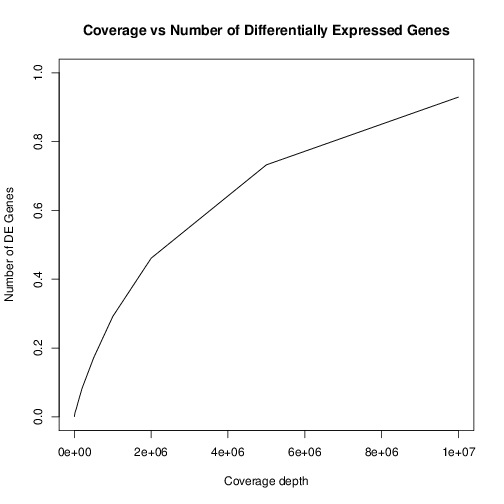
\includegraphics[width=0.4\textwidth]{./img/coverage.png}
      \end{center}
    \end{figure}
    \pause
    \item \textbf{Your mileage may vary!}
    \item \tiny{See Kliebenstein, (2012) FIPS: “Exploring the Shallow End;
                Estimating Information Content in Transcriptomics Studies.”}
  \end{itemize}
\end{frame}

\begin{frame}{Sequence analysis}
  \begin{itemize}
    \item Data is rawer now than with microarrays
    \begin{itemize}
      \item Needs significant computational resources
      \item At large scale, can be a bottleneck
    \end{itemize}
    \pause
    \item Have developed pipelines to do this efficiently
    \item \url{https://github.com/kdmurray91/RNAseqPipeline}
    \item \url{https://github.com/pedrocrisp/NGS-pipelines}
  \end{itemize}
\end{frame}

\begin{frame}{Sequence analysis pipeline}
  \begin{columns}[t]
    \column{0.4\textwidth}
      \begin{figure}[h]
        \begin{center}
          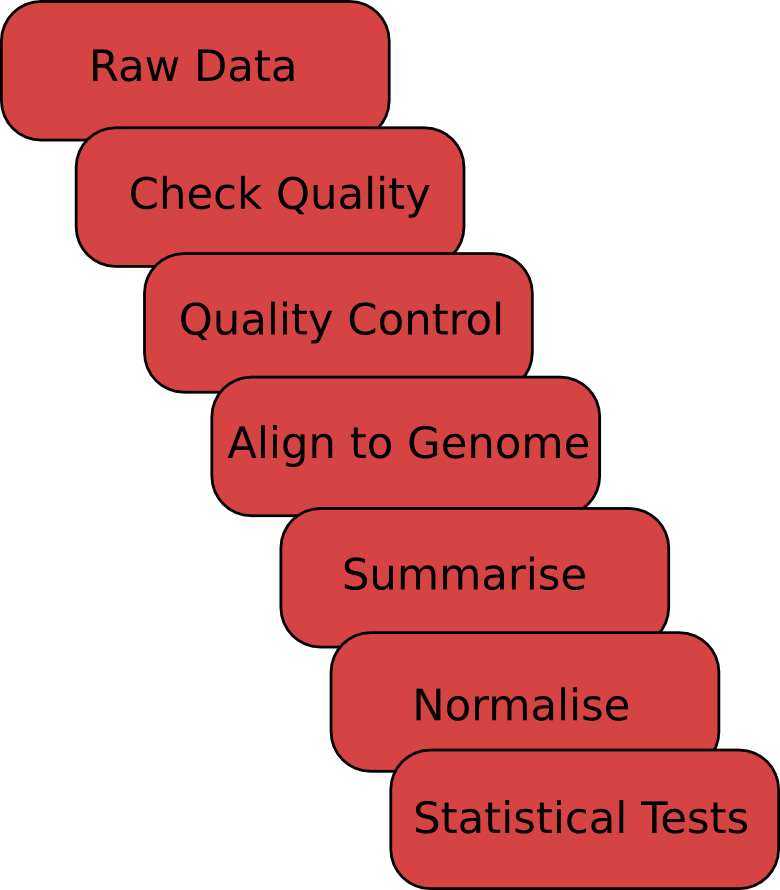
\includegraphics[width=0.8\textwidth]{img/informaticsFD.png}
        \end{center}
      \end{figure}
    \column{0.5\textwidth}
      \begin{itemize}
        \item \texttt{fastqc}
        \item \texttt{scythe}
        \item \texttt{sickle}
        \item \texttt{subread}/\texttt{subjunc}
        \item \texttt{featurecounts}
        \item \texttt{edgeR}
          \begin{itemize}
            \item \texttt{TMM} normalisation
            \item \texttt{exactTest} or \texttt{glmFit}
            \item Also using \texttt{limma}'s \texttt{voom}
          \end{itemize}
        \item \texttt{R} scripts for post-analysis
          \begin{itemize}
            \item \texttt{GOseq}
          \end{itemize}
          \item Diagnostic plots \textbf{highly recommended!}
      \end{itemize}
  \end{columns}
\end{frame}

\begin{frame}{Pipeline performance}
  \begin{itemize}
    \item Outperforms others by $>2-3$x
  \end{itemize}
  \begin{figure}[h]
    \begin{center}
      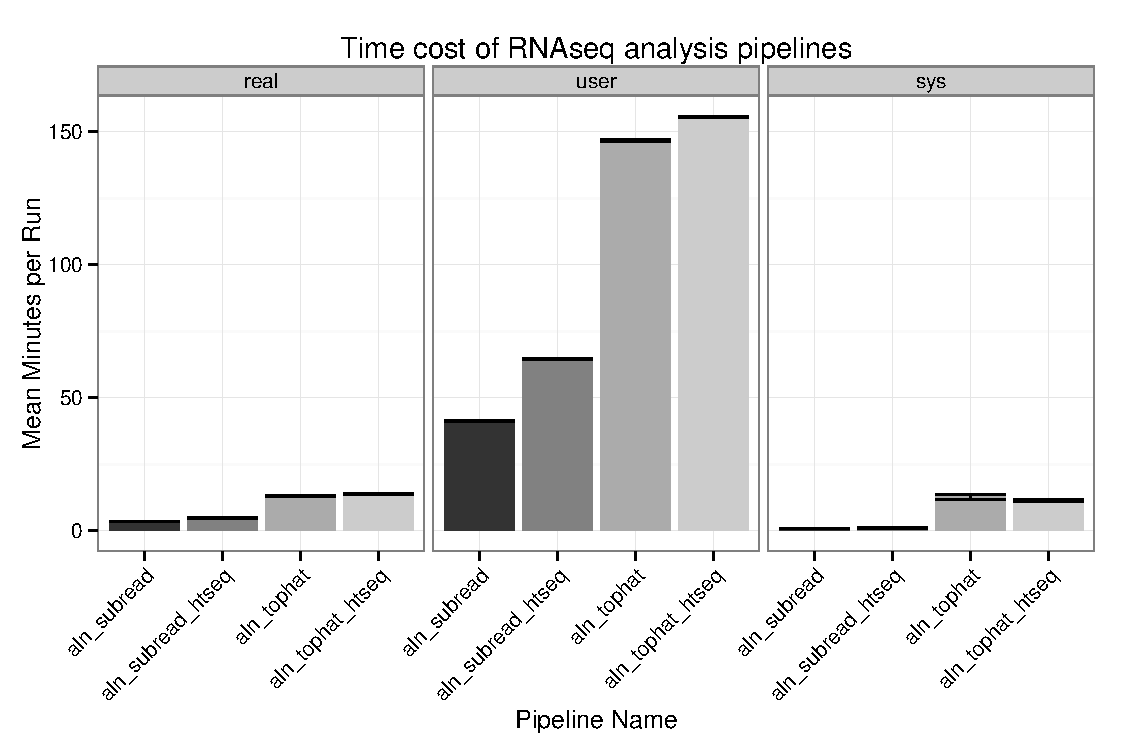
\includegraphics[width=\textwidth]{img/pltimes.pdf}
    \end{center}
  \end{figure}
\end{frame}<++>


\begin{frame}{MDS Plots save time!}
  \begin{itemize}
    \item If your reps don't cluster, time to cry into beer.
  \end{itemize}
  \begin{figure}[h]
    \begin{center}
      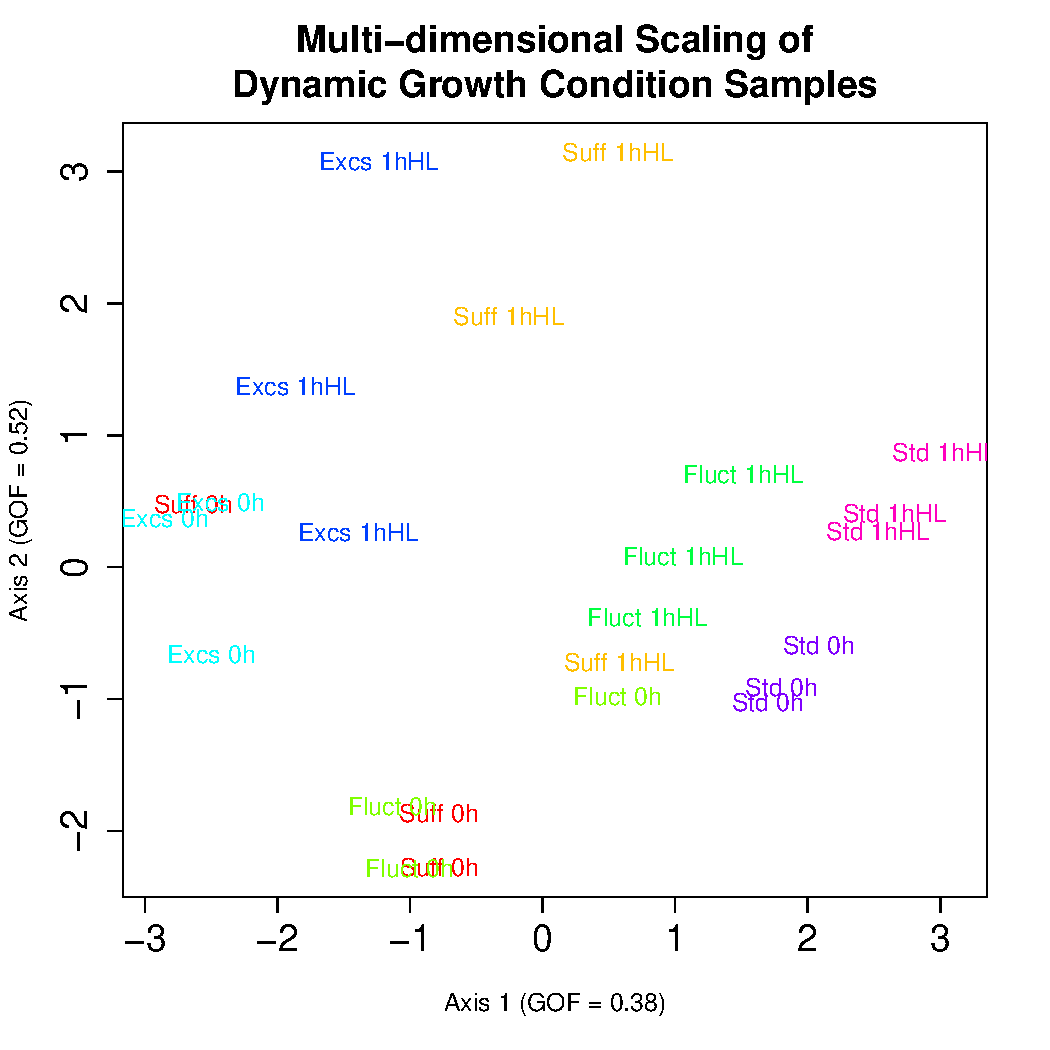
\includegraphics[width=0.6\textwidth]{img/txv-res-plotmds.pdf}
    \end{center}
  \end{figure}
\end{frame}

\begin{frame}{Existing DNA variation pipelines}
  \begin{itemize}
    \item Genotyping-by-sequencing
      \begin{itemize}
        \item Reference \& \textit{de-novo} analysis
        \item Porting to NCI NF
        \item Currently manual, working to automate
        \item Processed $>5000$ samples
      \end{itemize}
    \item Reference-based genotype calling
      \begin{itemize}
        \item Pipelines exist
        \item Not used a lot, requires deeper coverage
        \item See Norman's talk yesterday
      \end{itemize}
  \end{itemize}
\end{frame}

\begin{frame}{Novel algorithms for DNA variaiton}
  \begin{itemize}
    \item My PhD topic
  \pause
    \item Our wish-list:
    \begin{itemize}
      \item Reference \& alignment free
      \item Tolerates any sequencing kind
      \item Works with ``wide and shallow'' experiments: e.g. 1000 samples at
            1x
    \end{itemize}
  \pause
    \item e.g: gearing up to sequence 7500+ Eucalyptus, generating over 10 TB
      \textbf{raw} sequence data.
  \pause
    \item $k$-mer analysis: analyse $k$-length words of sequence
    \begin{itemize}
      \item Fast
      \item Constant-memory (with \texttt{khmer})
      \item Scaleable (linear time w/ number of samples)
      \item Parallelisable (within \& across nodes)
    \end{itemize}
  \end{itemize}
\end{frame}

\begin{frame}{Thanks}
      \begin{itemize}
        \item Borevitz lab (Norman, Justin, Megan, Steve)
        \item Pogson lab (Pete Crisp)
        \item Genome Discovery Unit
        \item Slides at \url{git.io/vfAof}
      \end{itemize}
\end{frame}

\begin{frame}{Grab-bag of capabilities}
  \begin{itemize}
    \item Confirm genotype using RNAseq reads
    \item Check technical reps are true
  \end{itemize}
\end{frame}

\end{document}
